
\section{Donaldson 的量子范畴}\label{sec:12-6}

\paragraph{辛微分同胚。}
研究\BookRecordIndex{T0229}量子上同调的\BookRecordIndex{T0132}弗洛尔同调方法可以沿两个方向推广。为简单起见，假设\BookRecordIndex{T0358}辛流形
$(M,\omega)$ 紧、单连通且单调。此时由式~\eqref{eq:12-1-2} 和
\eqref{eq:12-1-6}，\BookRecordIndex{T0131}弗洛尔连接轨道的能量由其指标控制（比较例~\ref{ex:8-6-8}）。所以
不必使用 Novikov 环，而可以用整数系数定义弗洛尔上同调群。代价是这些群现在只带模
$2N$ 分次，其中 $N$ 是最小 Chern 数。事实上，把分次约化为模 $2$ 很有用，这样便无须
为归一化分次作额外选择。归根结底，对每个辛微分同胚 $\phi$，都可以定义一个带模 $2$
分次的弗洛尔上同调群 $\operatorname{HF}^*(\phi)$，其 Euler 示性数
\[
  \chi\bigl(\operatorname{HF}^*(\phi)\bigr)=L(\phi)
\]
是 $\phi$ 的 \BookRecordIndex{T0032}Lefschetz 数。

生成弗洛尔复形的\BookRecordIndex{T0233}临界点现在是 $\phi$ 的不动点；假设它们都非退化。连接轨道则是满足
\[
  \phi(u(s,1))=u(s,0),\qquad s\in\mathbb R,
\]
的 $J$-全纯映射 $u:\mathbb R\times[0,1]\to M$。可以把它们看作辛纤维丛
\[
  P\longrightarrow\mathbb R\times S^1
\]
的 $J$-全纯截面；该丛以 $M$ 为纤维，绕 $S^1$ 的\BookRecordIndex{T0164}和乐为 $\phi$。若有退化不动点，就必须
像第~\ref{sec:12-1} 节那样选取\BookRecordIndex{T0157}哈密顿扰动。所得弗洛尔上同调群与定义时所用的\BookRecordIndex{T0157}哈密顿扰动
和\BookRecordIndex{T0088}殆复结构无关。（更多细节见 Floer \srcite{116}、Floer--Hofer--Salamon
\srcite{119} 与 Dostoglou--Salamon \srcite{90}。）由于 $M$ 单连通，每条\BookRecordIndex{T0361}辛同痕
$\{\phi_s\}_{0\leq s\leq1}$ 都决定一个同构
\[
  \operatorname{HF}^*(\phi_0)\longrightarrow\operatorname{HF}^*(\phi_1).
\]
正如注~\ref{rem:12-5-5} 所指出的，这个同构一般依赖于\BookRecordIndex{T0361}辛同痕的同伦类。对任意两个辛
微分同胚 $\phi,\psi$，还有自然同构
\[
  \operatorname{HF}^*(\phi)
  \longrightarrow
  \operatorname{HF}^*(\psi\circ\phi\circ\psi^{-1}).
\]
此外，按照 Donaldson 的说法，还存在形变\BookRecordIndex{T0228}量子杯积的类似物，即一个斜对称且结合的配对
\[
  \operatorname{HF}^*(\phi)\otimes\operatorname{HF}^*(\psi)
  \longrightarrow
  \operatorname{HF}^*(\psi\circ\phi).
\]
它可以用辛纤维丛 $P\to S$ 的 $J$-全纯截面定义，其中 $P$ 的纤维为 $M$，而 $S$ 是一个
带三个穿孔的二维球面；绕这三个穿孔的\BookRecordIndex{T0164}和乐分别共轭于
$\phi,\psi,\psi\circ\phi$。这个乘积结构可以解释为一个范畴：对象是 $M$ 的辛微分同胚，
从 $\phi$ 到 $\psi$ 的态射是弗洛尔上同调群
\[
  \operatorname{HF}^*(\psi\circ\phi^{-1})
\]
的元素，两个态射的复合由量子积给出。

现在取 $\psi=\operatorname{id}$。由第~\ref{sec:12-1} 节的讨论，在单调情形，弗洛尔
上同调群同构于通常上同调群：
\[
  \operatorname{HF}^*(\operatorname{id})
  =\operatorname{QH}^*(M)=H^*(M),
\]
其中分次以 $2$ 为周期。所以 $M$ 的上同调作用在 $\phi$ 的弗洛尔上同调上：
\[
  H^*(M)\otimes\operatorname{HF}^*(\phi)
  \longrightarrow\operatorname{HF}^*(\phi).
\]
在这种情形，还可以用另一种方式理解量子积结构。具体地，可以用余维 $k$ 的子流形（或
\BookRecordIndex{T0337}伪循环）$V\subset M$ 表示一个次数为 $k$ 的上同调类，再让 $V$ 与构造
$\phi$ 的弗洛尔上同调群时出现的连接轨道空间相交。更一般地，可以让这些连接轨道空间与
道路空间
\[
  \Omega_\phi:=\{\gamma:[0,1]\to M\mid \phi(\gamma(1))=\gamma(0)\}
\]
的有限维子流形相交，从而得到（低次数）上同调 $H^*(\Omega_\phi)$ 在
$\operatorname{HF}^*(\phi)$ 上的作用。

进一步特化到 $\phi=\operatorname{id}$，便可看出上述乘积构造与
第~\ref{sec:12-2} 节的\BookRecordIndex{T0217}裤形乘积一致；因此在这种情形，Donaldson 范畴约化为 $M$ 的\BookRecordIndex{T0229}量子
上同调。

\begin{remark}\label{rem:12-6-1}
到目前为止，人们只对少数例子计算出了辛微分同胚的\BookRecordIndex{T0132}弗洛尔同调群。即使在二维，这个问题
也颇为非平凡。Seidel 在 \srcite{361} 中计算了黎曼曲面 $\Sigma$ 的 Dehn 扭转之弗洛尔
上同调；又在 \srcite{369} 中证明，可以把恒等映射作为 $H^*(\Sigma)$-模与所有其他映射
类区分开来：如果 $\phi$ 不与恒等映射（辛）同痕，那么 $H^2(\Sigma)$ 在
$\operatorname{HF}^*(\phi)$ 上的作用平凡。Ralf Gautschi 在 \srcite{137,138} 中成功计算了
有限型辛微分同胚 $\phi:\Sigma\to\Sigma$ 的弗洛尔上同调群；所谓有限型，是指其 Thurston
分解中没有伪 Anosov 分支。Seidel 在 \srcite{362,370} 中发现了辛\BookRecordIndex{T0132}弗洛尔同调中的一个正合
序列，它类似于三维流形的瞬子\BookRecordIndex{T0132}弗洛尔同调中的 弗洛尔正合序列。他用这个正合序列计算了
辛四维流形 $X$ 上\BookRecordIndex{T0152}广义 Dehn 扭转 $\tau:X\to X$ 的弗洛尔上同调群，由此证明，在许多
情形中，这种 Dehn 扭转的平方 $\tau\circ\tau$ 不与恒等映射\BookRecordIndex{T0361}辛同痕。这个结果很不寻常，
因为 $\tau\circ\tau$ 总与恒等映射光滑同痕。（\BookRecordIndex{T0152}广义 Dehn 扭转 $\tau$ 本身在 $X$ 的
上同调上有非平凡作用。）在这项工作中，弗洛尔上同调上的乘积结构起着关键作用。

Fukaya 在 \srcite{125} 中研究了链\BookRecordIndex{T0072}层次的乘积结构，并发现了其底\BookRecordIndex{T0072}层的 $A_\infty$ 结构。
Seidel 在较近期的工作 \srcite{366,367} 中继续研究 Fukaya $A_\infty$ 范畴；这些范畴
似乎是理解镜像对称之同调版本的基础。

\paragraph{\BookRecordIndex{T0381}映射圆。}
当\BookRecordIndex{T0358}辛流形 $M$ 是如下\BookRecordIndex{T0246}模空间时，Donaldson 乘积结构尤其有趣：设 $\Sigma$ 是一个高亏格
黎曼曲面，$P\to\Sigma$ 是结构群为 $\operatorname{SO}(3)$ 的非平凡主丛，令 $M_\Sigma$
为 $P$ 上平坦联络的\BookRecordIndex{T0246}模空间。此时，$\Sigma$ 的映射类群通过辛微分同胚
\[
  \phi_f:M_\Sigma\longrightarrow M_\Sigma
\]
作用在 $M_\Sigma$ 上，其中 $f:\Sigma\to\Sigma$ 是保定向微分同胚；我们可以考察这些
映射类所生成的弗洛尔上同调群 $\operatorname{HF}^*(\phi_f)$。另有一种替代构造，它以
三维流形的\BookRecordIndex{T0132}弗洛尔同调群及四维配边上的 Yang--Mills 瞬子为基础。每个微分同胚
$f:\Sigma\to\Sigma$ 都诱导一个\BookRecordIndex{T0381}映射圆
\[
  Y_f:=\Sigma\times\mathbb R/\sim,
\]
其中通过 $f$ 把 $\Sigma\times\{t\}$ 与 $\Sigma\times\{t+1\}$ 识别。这些三维流形决定
\BookRecordIndex{T0132}弗洛尔同调群 $\operatorname{HF}^*(Y_f)$；它由 $Y_f$ 上的平坦
$\operatorname{SO}(3)$-联络和 $Y_f\times\mathbb R$ 上的反自对偶瞬子构造。Atiyah 与
Floer 猜想、Dostoglou--Salamon \srcite{92} 证明了自然同构
\[
  \operatorname{HF}^*(\phi_f)\cong\operatorname{HF}^*(Y_f).
\]
在 Floer--Donaldson 理论中，有配对
\[
  \operatorname{HF}^*(Y_f)\otimes\operatorname{HF}^*(Y_g)
  \longrightarrow\operatorname{HF}^*(Y_{gf}),
\]
它由四维流形 $X$ 上的反自对偶瞬子决定；$X$ 以带三个穿孔的球面 $S$ 为底，以 $\Sigma$
为纤维，并且\BookRecordIndex{T0164}和乐分别为 $f,g,gf$。上述同构保持这两个乘积；这一点由 Salamon
在 \srcite{352} 中证明。

取 $g=\operatorname{id}$ 会得到一个有趣的特例。这时，$\phi_g$ 的辛弗洛尔上同调，进而
$Y_g$ 的瞬子弗洛尔上同调，等于以 $4$ 为周期的\BookRecordIndex{T0246}模空间 $M_\Sigma$ 的通常上同调。因此，
$M_\Sigma$ 的\BookRecordIndex{T0229}量子上同调作用在 $Y_f$ 的弗洛尔上同调上：
\[
  \operatorname{QH}^*(M_\Sigma)\otimes\operatorname{HF}^*(Y_f)
  \longrightarrow\operatorname{HF}^*(Y_f).
\]
$M_\Sigma$ 的上同调（以及\BookRecordIndex{T0229}量子上同调）已经得到充分理解，并与黎曼曲面 $\Sigma$ 本身的
同调密切相关；比较例~\ref{ex:11-1-15}。例如，有一个同态的普适构造
\[
  \mu:H_1(\Sigma)\longrightarrow H^3(\mathcal B_\Sigma^*),
  \qquad
  \mathcal B_\Sigma^*:=\mathcal A_\Sigma^*/\mathcal G_\Sigma,
\]
其中 $\mathcal B_\Sigma^*$ 表示 $P\to\Sigma$ 上不可约联络模\BookRecordIndex{T0153}规范等价的无限维位形空间。
这就是 Donaldson 的 $\mu$-映射。粗略地说，它可描述为斜积
\[
  \mu(\gamma)=-\frac14p_1(\mathcal P)/\gamma,
\]
其中 $p_1(\mathcal P)\in H^4(\mathcal B_\Sigma^*\times\Sigma)$ 表示普适
$\operatorname{SO}(3)$-丛
$\mathcal P\to\mathcal B_\Sigma^*\times\Sigma$ 的第一 Pontryagin 类。更明确地说，
$H^3(M_\Sigma)$ 中所诱导的上同调类由余维三子流形 $V_\gamma\subset M_\Sigma$ 表示；它
由绕 $\gamma$ 的\BookRecordIndex{T0164}和乐平凡的那些平坦联络组成。总而言之，有以下两个图：
\[
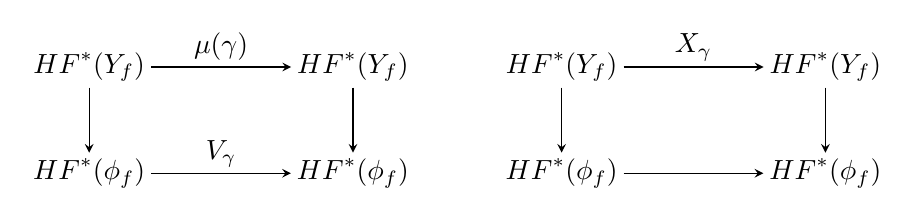
\begin{tikzpicture}[baseline=(current bounding box.center),>=stealth,
  every node/.style={inner sep=2pt}]
  \node (a1) at (0,1.35) {$\operatorname{HF}^*(Y_f)$};
  \node (a2) at (3.35,1.35) {$\operatorname{HF}^*(Y_f)$};
  \node (a3) at (0,0) {$\operatorname{HF}^*(\phi_f)$};
  \node (a4) at (3.35,0) {$\operatorname{HF}^*(\phi_f)$};
  \draw[->] (a1) -- node[above] {$\mu(\gamma)$} (a2);
  \draw[->] (a3) -- node[above] {$V_\gamma$} (a4);
  \draw[->] (a1) -- (a3);
  \draw[->] (a2) -- (a4);
  \node (b1) at (6.0,1.35) {$\operatorname{HF}^*(Y_f)$};
  \node (b2) at (9.35,1.35) {$\operatorname{HF}^*(Y_f)$};
  \node (b3) at (6.0,0) {$\operatorname{HF}^*(\phi_f)$};
  \node (b4) at (9.35,0) {$\operatorname{HF}^*(\phi_f)$};
  \draw[->] (b1) -- node[above] {$X_\gamma$} (b2);
  \draw[->] (b3) -- (b4);
  \draw[->] (b1) -- (b3);
  \draw[->] (b2) -- (b4);
\end{tikzpicture}
\]
每个图中的竖直箭头都是 \srcite{92} 的自然同构。左图的水平映射，是用适当子流形与连接
轨道的\BookRecordIndex{T0246}模空间相交、把这些\BookRecordIndex{T0246}模空间截低而定义的；右图的水平映射则由用配边定义的乘积结构
给出。例如，类 $\gamma\in H_1(\Sigma)$ 决定一个自然配边 $X_\gamma$，其边界为
\[
  \partial X_\gamma=(-Y_f)\cup Y_f.
\]
当然，在自然同构下，乘积的四种定义都应当一致。这些乘积结构之间的关系，在 Michael
Callaghan 关于 $M_\Sigma$ 的辛微分同胚（由分离型 Dehn 扭转诱导）之\BookRecordIndex{T0361}辛同痕问题的工作中
起着重要作用。遗憾的是，他的工作从未发表。

这些乘积结构在 Floer--Fukaya 构造中也起着重要作用；该构造为偶对 $(Y,\gamma)$ 给出
上同调群 $\operatorname{HFF}^*(Y,\gamma)$，其中 $Y$ 是三维流形、
$\gamma\in H_1(Y)$。另一方面，弗洛尔正合序列中的同态也可以用这些乘积结构来解释。

\paragraph{拉格朗日交。}
拉格朗日交的弗洛尔上同调中有类似结构；事实上，这正是 \BookRecordIndex{T0014}Donaldson 量子范畴构造的原始
背景。设 $M$ 如上，即紧、单连通且单调。对每一对满足 $H^1(L_i;\mathbb R)=0$ 的
\BookRecordIndex{T0219}拉格朗日子流形 $L_0,L_1$，都有弗洛尔上同调群 $\operatorname{HF}^*(L_0,L_1)$。此时
\BookRecordIndex{T0233}临界点是交点 $L_0\cap L_1$，连接轨道则是满足
\[
  u(s,0)\in L_0,
  \qquad u(s,1)\in L_1
\]
的 \BookRecordIndex{T0003}$J$-全纯曲线 $u:\mathbb R\times[0,1]\to M$。这是 Floer 在 \srcite{113} 中原始工作的
背景。弗洛尔上同调的 Euler 示性数现在是交数
\[
  \chi\bigl(\operatorname{HF}^*(L_0,L_1)\bigr)=L_0\cdot L_1.
\]
同样有由全纯三角形定义的配对
\[
  \operatorname{HF}^*(L_0,L_1)\otimes\operatorname{HF}^*(L_1,L_2)
  \longrightarrow\operatorname{HF}^*(L_0,L_2).
\]
Floer 在 \srcite{113} 中证明，只要 $\pi_2(M,L_0)=0$，
$\operatorname{HF}^*(L_0,L_0)$ 就同构于 $L_0$ 的通常上同调。在我们假设 $M$ 单连通的
情形，这个条件从不成立，相应断言仍是开放问题。Biran--Cornea 在 \srcite{44} 中把满足
$\operatorname{HF}^*(L_0,L_0)\cong H^*(L_0)$ 的\BookRecordIndex{T0219}拉格朗日子流形称为\emph{宽的}，把
$\operatorname{HF}^*(L_0,L_0)$ 消失的称为\emph{窄的}。在本书写作时，人们对这种二分仍
未充分理解。

这个乘法结构可以解释为一个量子范畴：对象是满足 $H^1(L;\mathbb R)=0$ 的\BookRecordIndex{T0219}拉格朗日
子流形 $L\subset M$，从 $L_0$ 到 $L_1$ 的态射是弗洛尔上同调群
$\operatorname{HF}^*(L_0,L_1)$ 的元素。上述辛微分同胚结构是它的特例，其中
\[
  M=N\times N,
  \qquad L_0=\Delta,
  \qquad L_1=\operatorname{graph}(\phi),
  \qquad L_2=\operatorname{graph}(\psi).
\]

把\BookRecordIndex{T0219}拉格朗日子流形解释为范畴的对象、把弗洛尔上同调群解释为态射空间的观点来自
Donaldson。后来 Fukaya 在链\BookRecordIndex{T0072}层次发现了底\BookRecordIndex{T0072}层的 $A_\infty$ 结构。所得范畴称为 \BookRecordIndex{T0021}Fukaya 范畴，
记作 $\mathcal F(M)$。即使在不会\BookRecordIndex{T0243}冒泡的简单情形，严格构造 \BookRecordIndex{T0021}Fukaya 范畴也涉及相当大量的
精细分析。例如，Seidel \srcite{371} 发展了计算仿射 Calabi--Yau 流形某些导出范畴
$D^b\mathcal F(M)$ 的技术。他的构造涉及对 Lefschetz 铅笔、消失循环和 Seidel 正合序列
作归纳论证。Fukaya--Seidel--Smith \srcite{131} 利用余切丛的 \BookRecordIndex{T0021}Fukaya 范畴取得了显著
成效。这里同样没有\BookRecordIndex{T0243}冒泡，却必须处理由非\BookRecordIndex{T0192}紧性造成的问题。一般情形见
Fukaya--Oh--Ohta--Ono \srcite{128}。Wehrheim 与 Woodward 在近期一系列论文
\srcite{414,415,416,417} 中证明了单调情形下 Donaldson 范畴关于拉格朗日对应的函子性。

\paragraph{Heegaard 分裂。}
拉格朗日交的弗洛尔理论与三维流形有如下联系。若 $Y$ 是同调三维球面，就在黎曼曲面
$\Sigma$ 上选取一个 Heegaard 分裂
\[
  Y=Y_0\cup Y_1.
\]
每个柄体 $Y_j$ 都在 $\Sigma$ 上平坦 $\operatorname{SU}(2)$-联络的（奇异）\BookRecordIndex{T0246}模空间
$M_\Sigma$ 中决定一个（奇异）\BookRecordIndex{T0219}拉格朗日子流形
$L_j=L_{Y_j}\subset M_\Sigma$。按照 Atiyah \srcite{20} 与 Floer 的观点，应当有自然同构
\[
  \operatorname{HF}^*(Y_0\cup Y_1)
  \cong\operatorname{HF}^*(L_0,L_1).
\]
和前面一样，有乘积结构
\[
  \operatorname{HF}^*(Y_0\cup Y_1)
  \otimes\operatorname{HF}^*(Y_1\cup Y_2)
  \longrightarrow\operatorname{HF}^*(Y_0\cup Y_2),
\]
它直接用适当四维配边上的 Yang--Mills 瞬子定义；在上述（猜想的）同构下，这两个乘积结构
应当相关。Katrin Wehrheim 在 \srcite{411,412,413} 中研究带拉格朗日边界条件的反自对偶
瞬子，并在这一猜想上取得了重要进展。作为中间步骤，这项工作在 Salamon--Wehrheim
\srcite{355} 中促成了带边三维流形的\BookRecordIndex{T0132}弗洛尔同调群之定义。（另一种设置可见 Fukaya
较早的工作 \srcite{126}。）

沿亏格为 $g$ 的黎曼曲面 $\Sigma$ 作 Heegaard 分裂，还会在 $g$ 重对称积
$\operatorname{Sym}^g\Sigma$ 中决定两个拉格朗日环面。从 \srcite{318} 开始的一长串论文中，
Ozsváth--Szabó 从他们的拉格朗日弗洛尔理论发展出一套强有力的新不变量，适用于低维流形
及纽结，称为 Heegaard--Floer 理论。他们又与若干合作者共同推进四维拓扑量子场论的构造；
参见 Lipshitz--Ozsváth--Thurston \srcite{247}。
\end{remark}
